\documentclass[a4paper, 10pt]{article}
\usepackage{scrextend}
\changefontsizes{9pt}
% Per-subject config for this repo. See vendor/template/course-config.tex.example
% for what each macro is used for.

\newcommand{\CourseCode}{2110473}
\newcommand{\CourseName}{Fault Tolerant Computing}
\newcommand{\StudentID}{6733172621}
\newcommand{\StudentName}{Patthadon Phengpinij}
\newcommand{\DefaultCollaborators}{Claude (for\,\LaTeX\,styling and grammar checking)}
\newcommand{\AssignmentLabel}{Homework}

\usepackage{../vendor/template/CEDT-Assignment-style}

\begin{document}
\subject
\asgntitle{8}{}{Week 10}{\StudentID\ \StudentName}{\DefaultCollaborators}

\begin{center}

	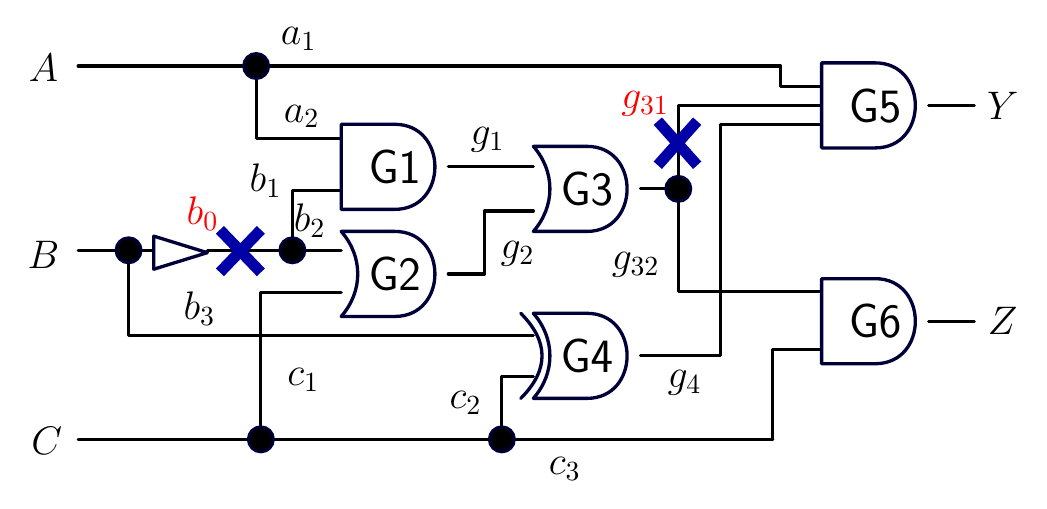
\begin{tikzpicture}[
			x=0.020cm, y=-0.020cm,
			wire/.style={
					draw=black,
					line width=1.15pt,
					line cap=round,
					line join=round
				},
			gate/.style={
					draw=blue!22!black,
					fill=white,
					line width=1.2pt,
					line join=round
				},
			dot/.style={
					circle,
					draw=blue!22!black,
					fill=black,
					line width=1pt,
					minimum size=0.32cm,
					inner sep=0pt
				},
			sig/.style={
					font=\Large,
					inner sep=0pt
				},
			gtext/.style={
					font=\sffamily\LARGE,
					inner sep=0pt
				},
			fault/.style={
					draw=blue!65!black,
					line width=4pt,
					line cap=butt
				}
		]

		% =========================================================
		% Common gate size parameters
		% =========================================================
		\def\gw{34}
		\def\gh{27}

		% Gate centers
		\coordinate (G1c) at (248,98);
		\coordinate (G2c) at (248,166);
		\coordinate (G3c) at (370,112);
		\coordinate (G4c) at (370,218);
		\coordinate (G5c) at (553,59);
		\coordinate (G6c) at (553,196);

		% =========================================================
		% Input wires and branches
		% =========================================================

		% Input A
		% Adjusted upper input to G5: y = 47
		\draw[wire]
		(47,34) -- (493,34)
		-- (493,47) -- (519,47);

		\draw[wire]
		(160,34) -- (160,80) -- (214,80);

		% Input B
		\draw[wire] (47,151) -- (95,151);
		\draw[wire] (129,151) -- (214,151);
		\draw[wire]
		(183,151) -- (183,113) -- (214,113);
		\draw[wire]
		(79,151) -- (79,205) -- (336,205);

		% Input C
		\draw[wire] (47,271) -- (488,271);
		\draw[wire]
		(163,271) -- (163,178) -- (214,178);
		\draw[wire]
		(316,271) -- (316,231) -- (336,231);
		\draw[wire]
		(488,271) -- (488,214) -- (519,214);

		% =========================================================
		% Intermediate wires
		% =========================================================

		% g1 : G1 -> G3
		\draw[wire] (282,98) -- (336,98);

		% g2 : G2 -> G3
		\draw[wire]
		(282,166) -- (305,166)
		-- (305,126) -- (336,126);

		% G3 output
		\draw[wire] (404,112) -- (428,112);

		% g31 : G3 -> G5, middle input y = 59
		\draw[wire]
		(428,112) -- (428,59) -- (519,59);

		% g32 : G3 -> G6
		\draw[wire]
		(428,112) -- (428,177) -- (519,177);

		% g4 : G4 -> G5
		% Adjusted lower input to G5: y = 71
		\draw[wire]
		(404,218) -- (455,218)
		-- (455,71) -- (519,71);

		% Outputs
		\draw[wire] (587,59) -- (616,59);
		\draw[wire] (587,196) -- (616,196);

		% =========================================================
		% Triangular buffer
		% =========================================================
		\draw[gate]
		(95,142) -- (95,163)
		-- (129,152.5) -- cycle;

		% =========================================================
		% G1 : AND gate
		% =========================================================
		\draw[gate]
		(214,71) -- (248,71)
		.. controls (282,71) and (282,125) .. (248,125)
		-- (214,125) -- cycle;

		% =========================================================
		% G2 : OR gate
		% =========================================================
		\draw[gate]
		(214,139)
		.. controls (230,139) and (240,139) .. (248,139)
		.. controls (282,139) and (282,193) .. (248,193)
		.. controls (240,193) and (230,193) .. (214,193)
		.. controls (228,177) and (228,155) .. (214,139)
		-- cycle;

		% =========================================================
		% G3 : OR gate
		% =========================================================
		\draw[gate]
		(336,85)
		.. controls (352,85) and (362,85) .. (370,85)
		.. controls (404,85) and (404,139) .. (370,139)
		.. controls (362,139) and (352,139) .. (336,139)
		.. controls (350,123) and (350,101) .. (336,85)
		-- cycle;

		% =========================================================
		% G4 : XOR gate
		% =========================================================
		\draw[gate]
		(336,191)
		.. controls (352,191) and (362,191) .. (370,191)
		.. controls (404,191) and (404,245) .. (370,245)
		.. controls (362,245) and (352,245) .. (336,245)
		.. controls (350,229) and (350,207) .. (336,191)
		-- cycle;

		% Additional XOR curve
		\draw[
			draw=blue!22!black,
			line width=1.2pt,
			line cap=round,
			line join=round
		]
		(328,191)
		.. controls (346,209) and (346,227) .. (328,245);

		% =========================================================
		% G5 : Three-input AND gate
		% Input wires at y = 47, 59, 71
		% =========================================================
		\draw[gate]
		(519,32) -- (553,32)
		.. controls (587,32) and (587,86) .. (553,86)
		-- (519,86) -- cycle;

		% =========================================================
		% G6 : AND gate
		% =========================================================
		\draw[gate]
		(519,169) -- (553,169)
		.. controls (587,169) and (587,223) .. (553,223)
		-- (519,223) -- cycle;

		% =========================================================
		% Junction dots
		% =========================================================
		\foreach \p in {
				(160,34),
				(79,151),
				(183,151),
				(163,271),
				(316,271),
				(428,112)
			}{
				\node[dot] at \p {};
			}

		% =========================================================
		% Blue fault markers
		% =========================================================

		% Fault b_0
		\draw[fault] (137,138) -- (163,165);
		\draw[fault] (137,165) -- (163,138);

		% Fault g_{31}
		\draw[fault] (415,69) -- (440,97);
		\draw[fault] (415,97) -- (440,69);

		% =========================================================
		% Gate labels
		% =========================================================
		\node[gtext] at (248,98)  {G1};
		\node[gtext] at (248,166) {G2};
		\node[gtext] at (370,112) {G3};
		\node[gtext] at (370,218) {G4};
		\node[gtext] at (553,59)  {G5};
		\node[gtext] at (553,196) {G6};

		% =========================================================
		% External input/output labels
		% =========================================================
		\node[sig] at (25,35) {$A$};
		\node[sig] at (25,154) {$B$};
		\node[sig] at (27,272) {$C$};

		\node[sig] at (634,59) {$Y$};
		\node[sig] at (634,196) {$Z$};

		% =========================================================
		% Path labels with subscripts
		% =========================================================

		% A paths
		\node[sig] at (187,17) {\( a_1 \)};
		\node[sig] at (189,66) {\( a_2 \)};

		% B paths
		\node[sig,text=red] at (126,128) {\( b_0 \)};
		\node[sig] at (166,107) {\( b_1 \)};

		% Moved b_2 left and slightly upward
		% to increase clearance from gate G2
		\node[sig] at (194,132) {\( b_2 \)};

		\node[sig] at (124,188) {\( b_3 \)};

		% C paths
		\node[sig] at (190,233) {\( c_1 \)};
		\node[sig] at (293,248) {\( c_2 \)};
		\node[sig] at (356,290) {\( c_3 \)};

		% Gate output paths
		\node[sig] at (307,81) {\( g_1 \)};
		\node[sig] at (326,153) {\( g_2 \)};
		\node[sig,text=red] at (407,58) {\( g_{31} \)};
		\node[sig] at (401,160) {\( g_{32} \)};
		\node[sig] at (432,235) {\( g_4 \)};

	\end{tikzpicture}
\end{center}

% ================================================================================ %
%                                    Problem 01                                    %
% ================================================================================ %
\begin{problem}
Find the test input when \( b_0 \) is stuck-at 0 fault.
\end{problem}

\begin{solution}
	\noindent Circuit functions:
	\begin{align*}
		G1 & = AB                \\
		G2 & = B+C               \\
		G3 & = AB+B+C = B+C      \\
		G4 & = B\oplus C         \\
		Y  & = A\cdot G3\cdot G4 \\
		Z  & = G3\cdot C
	\end{align*}

	\begin{itemize}
		\item \textbf{Activate:} \( b_0 \) s-a-0 \( \Rightarrow \) need \( B=1 \).
		\item \textbf{Propagate:} through G2 needs \( c_1=C=0 \) (then \( G3 \): good \( 1 \), faulty \( 0 \)).
		      Through G5 needs \( A=1 \) and \( g_4=B\oplus C=1 \) (true for \( B=1,C=0 \)).
		      (Through G6 is impossible since \( C=0 \).)
	\end{itemize}
	\[ \boxed{ABC = 110} \quad \Rightarrow \quad Y_{good}=1,\ Y_{faulty}=0. \]
\end{solution}
% ================================================================================ %

% ================================================================================ %
%                                    Problem 02                                    %
% ================================================================================ %
\begin{problem}
How many faults can be tested by the test input on 1?
\end{problem}

\begin{solution}
	\noindent Good values under \( ABC=110 \): \( A=a_1=a_2=1 \), \( B=b_0=b_1=b_2=b_3=1 \),
	\( C=c_1=c_2=c_3=0 \), \( g_1=g_2=g_{31}=g_{32}=g_4=1 \), \( Y=1 \), \( Z=0 \).
	Simulating each single stuck-at (opposite) fault, the detected ones are
	\[
		A/0,\ a_1/0,\ B/0,\ b_0/0,\ b_3/0,\ C/1,\ c_2/1,\ c_3/1,\ g_{31}/0,\ g_4/0,\ Y/0,\ Z/1
	\]
	so \( \boxed{12 \text{ faults}} \) are detected (13 if the unlabeled G3 output stem s-a-0 is counted).
	The faults \( a_2/0, b_1/0, b_2/0, c_1/1, g_1/0, g_2/0, g_{32}/0 \) are not detected
	(G3 is still kept at 1 by the other input, or \( Z \) is blocked by \( C=0 \)).
\end{solution}
% ================================================================================ %

% ================================================================================ %
%                                    Problem 03                                    %
% ================================================================================ %
\begin{problem}
Find the test input when \( g_{31} \) is stuck-at 1 fault.
\end{problem}

\begin{solution}
	\begin{itemize}
		\item \textbf{Activate:} \( g_{31} \) s-a-1 \( \Rightarrow \) need \( G3=B+C=0 \), i.e.\ \( B=0,\ C=0 \).
		\item \textbf{Propagate:} through G5 needs \( A=1 \) and \( g_4=B\oplus C=1 \),
		      but \( B=C=0 \) gives \( g_4=0 \). Contradiction.
	\end{itemize}
	Hence \( \boxed{\text{no test input exists}} \): \( g_{31} \) s-a-1 is undetectable (redundant),
	since \( Y = A(B+C)(B\oplus C) = A(B\oplus C) \) already does not depend on \( g_{31} \).
\end{solution}
% ================================================================================ %

% ================================================================================ %
%                                    Problem 04                                    %
% ================================================================================ %
\begin{problem}
What happens when applying the test input on 1 to the multiple faults of \( b_0 \) (s-a-0) and \( g_{31} \) (s-a-1)?
\end{problem}

\begin{solution}
	\noindent With \( ABC=110 \) and both faults: \( b_0=0 \Rightarrow g_1=0,\ g_2=C=0 \Rightarrow G3=0 \),
	so \( g_{32}=0 \), but \( g_{31} \) is stuck at 1. Then
	\[ Y = a_1\cdot g_{31}\cdot g_4 = 1\cdot1\cdot1 = 1, \qquad Z = 0\cdot0=0, \]
	which equals the good output. The undetectable \( g_{31} \) s-a-1 \textbf{masks} \( b_0 \) s-a-0,
	so the test \( 110 \) no longer detects \( b_0 \) s-a-0. In fact, with both faults
	\( Y=A(B\oplus C) \) and \( Z=C \), identical to the fault-free circuit, so this multiple
	fault cannot be detected by any input.
\end{solution}
% ================================================================================ %

\end{document}
